\section{Method}
\label{sec:method}

\begin{figure*}[t]
    \centering
    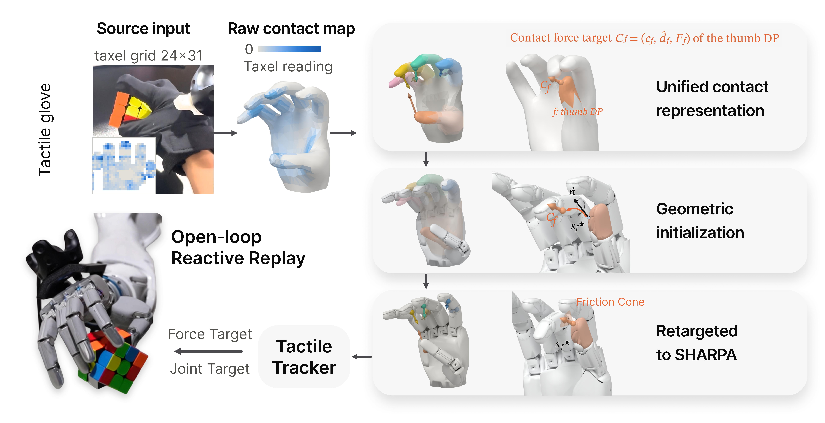
\includegraphics[width=0.8\linewidth]{figs/fig_source_data.pdf}
    \caption{\textbf{\ours overview.} Video, glove, and motion capture are converted into a unified hand--contact representation, a MANO mesh with one contact force target per semantic link (\cref{sec:method:uhcr}). Geometric initialization maps human joint angles to the robot skeleton, followed by contact-anchored retargeting that aligns the corresponding robot pads with the contact force targets (\cref{sec:method:retarget}). Joint and contact force targets are replayed by a tactile tracking controller (\cref{sec:method:replay}) on hardware.}
    \label{fig:pipeline}
\end{figure*}

Given a demonstration with hand pose and contact, \ours (\cref{fig:pipeline}) produces a robot trajectory that reproduces its \fca, not only its kinematics. Per frame we solve for the hand pose $q = (t, R, \theta)
\in \mathbb{R}^3 \times \mathrm{SO}(3) \times \mathbb{R}^{N}$: wrist position, wrist rotation as an axis--angle vector, and the $N$ joint angles ($N{=}22$ for the SHARPA Wave), without a physics simulator or object model as input. Every \emph{contact force target} is bound to the hand surface, so deformable and articulated objects can be handled without additional burden. Hats ($\hat{\phantom{s}}$) denote unit vectors, $q^{\star}$ denotes the optimal solution of a frame, $q^{-}$ denotes the previous frame's solution.
% \akash{what is this? unclear: robot point that corresponds to one?}
\subsection{Unified Hand--Contact Representation}
\label{sec:method:uhcr}


Every data source is reduced to three components (\cref{fig:regions}): a MANO~\citep{mano} hand mesh sequence, a vocabulary of semantic links (3 regions per finger, 15 finger regions plus the palm region, see \cref{app:details} for details) shared by every source and every robot, and at most one \emph{contact force target} per link and frame, denoted by $C_f = (c_f, \hat{d}_f, F_f)$, where $f$ is the finger link and $\mathcal{F}$ the full robot link set. The center of pressure $c_f \in \Rb^3$ is constrained onto link surface $f$, $\hat{d}_f$ denotes a unit push direction into the object, and $F_f \geq 0$ denotes the force magnitude. Video does not provide contact force, so we synthesize it from the contact predictions. Source-specific processing into the shared representation is detailed in \cref{app:data_unification}.

\subsection{Vid-HACO: Contact from Monocular Video}
\label{sec:method:vidhaco}

For monocular video, we introduce Vid-HACO, a video-based hand–object contact estimation model that predicts contact probabilities for all 778 MANO vertices, enabling video demonstrations to be converted into our unified hand–contact representation. Given an 8-frame clip ending at frame $t$, Vid-HACO uses hand crops obtained from HaWoR~\citep{hawor}, a world-frame extension of HaMeR~\citep{hamer}. A video-pretrained V-JEPA 2.1 ViT-L encoder \citep{vjepa21} and a DPT decoder \citep{dpt} extract multi-scale features. Two prediction heads estimate vertex-level contact logits and a frame-level binary contact indicator, respectively. Temporal context helps distinguish contact transitions during approach, grasp, and release.

Following HACO~\citep{haco}, we use a 10\,mm distance threshold to label vertices as contacting the touched surface and set the probability threshold to 0.52 for contact prediction. We train on 1.55M frames from 12 datasets spanning egocentric, third-person, and web views, holding out 10\% of each dataset for validation. We fine-tune the encoder end to end with HACO's class-balanced vertex loss~\citep{cbloss} and an additional binary cross-entropy loss on the frame head, retaining contact-free frames during training. Dataset and implementation details appear in \cref{app:vidhaco}.

\subsection{Contact-Anchored Retargeting}
\label{sec:method:retarget}

\nbf{Geometric initialization} We first retarget human joint angles directly to the robot skeleton using closed form approaches (i.e., without optimization) and adjust the wrist pose to align the robot and human fingertips in 3D. Because the thumb joint ranges and motion axes cannot be mapped directly, we compute its pose using a fixed affine transformation derived from its bone directions and pad normal (\cref{app:init}). The resulting configuration $q^{\mathrm{init}}$ is deterministic and warm starts the following optimization (\cref{fig:init}).

%\nbf{Geometric initialization} We first copy the human skeleton onto the robot in closed form, \akash{what does copying in closed form mean?} \todo{here I'm trying to say not running any optimization, direct copy or linear transformation, let me rephrase} and adjust wrist pose so the robot fingertips align with the human's in 3D. The thumb, whose ranges and axes admit no angle copy, uses a fixed affine map from its human bone directions and pad normal (\cref{app:init}). The result $q^{\mathrm{init}}$ is deterministic and enters the solve only as half of the warm start (\cref{fig:init}).

\nbf{Problem formulation} For each frame, we optimize the robot joint configuration $q^\star$ by solving:
\begin{align}
\label{eq:objective}
q^{\star} = \arg\min_{q \in \mathcal{Q}} \; &E_{\mathrm{contact}}(q) + E_{\mathrm{style}}(q) + E_{\mathrm{smooth}}(q)\nonumber\\ + &E_{\mathrm{collision}}(q),
\end{align}
where $E_{\mathrm{contact}}$ aligns the robot's fingertip pads with \fca, $E_{\mathrm{style}}$ encourages unconstrained (free) fingers to mimic human poses, $E_{\mathrm{smooth}}$ maintains smooth joint movements, while $E_{\mathrm{collision}}$ prevents robot self-collisions and object penetration. The feasible set $\mathcal{Q}$ enforces joint position and velocity limits across all joints. A single set of loss weights $w$ is used across all motion sequences. The weights appear inside each energy term below and are listed in \cref{tab:solver} of \cref{app:details}.
% \nbf{Problem formulation} Per frame we seek
% \begin{equation}
% \label{eq:objective}
% q^{\star} \;=\; \argmin_{q \in \mathcal{Q}}\; E_{\mathrm{con}}(q) + E_{\mathrm{sty}}(q) + E_{\mathrm{smo}}(q) + E_{\mathrm{col}}(q),
% \end{equation}
% where $E_{\mathrm{con}}$(contact group) places the robot's pads on the contact force anchors. $E_{\mathrm{sty}}$(style group)  makes the free fingers imitate the human, $E_{\mathrm{smo}}$(smoothness group)  keeps the step from the previous frame small, and $E_{\mathrm{col}}$(collision group)  penalizes robot self-collision and object penetration. The feasible set $\mathcal{Q}$ holds joint limits and velocity caps for each joints. One set of weights $w_{\bullet}$ serves all sources (\cref{tab:solver}).

\nbf{Contact group} Each robot contact region $f \in \mathcal{F}$ on the pad surface $\mathcal{S}_f(q)$ is defined by its 3D position $s_f(q)$ and outward surface normal $\hat{n}(s)$, which specifies the central axis of its friction cone. To prevent physically unrealistic assignments (e.g., satisfying a fingertip contact using a mid-link surface), we select an optimal contact point $s^{*}_f(q)$ by balancing geometric contact proximity against human contact preferences:
\begingroup\setlength{\abovedisplayskip}{3pt}\setlength{\belowdisplayskip}{3pt}\setlength{\abovedisplayshortskip}{1pt}\setlength{\belowdisplayshortskip}{1pt}
\begin{equation}\label{eq:selector}s^*_f(q) = \argmin\nolimits_{s \in \mathcal{S}_f(q)} \|s - c_f\|^2 + \alpha_f \|s - T_f\psi_f\|^2.\end{equation}\endgroup
Here, $c_f$ is the target contact location and $\psi_f$ is the human contact preference remapped onto the robot link: the point on the link's palmar centerline at the same fractional position $u_f$ at which the human touched the corresponding finger segment, $u_f = \mathrm{clip}\big(\tfrac{(c_f - j_0)\cdot(j_1 - j_0)}{\|j_1 - j_0\|^2},\, 0,\, 1\big)$, where $j_0$ and $j_1$ are the joints bounding that segment (e.g., DIP and fingertip for the distal region). The link pose $T_f(q)$ maps $\psi_f$ into the world frame. Because $s$ and $\psi_f$ lie on the same rigid link, the second term acts as a fixed offset in the link frame that guides the selection of $s^{*}_f(q)$. Once selected, $s^{*}_f(q)$ is evaluated in the total contact objective $E_{\mathrm{contact}}(q)$:

\begin{equation}
\label{eq:contact}
\begin{split}
E_{\mathrm{contact}}(q) = {}& \sum_{f \in \mathcal{F}} \rho_f^2 \Big[\, w_{\mathrm{c}}^2 \Big( \underbrace{\big\| s^{*}_f(q) - c_f \big\|^2}_{\text{contact reach}} \\
& + \underbrace{\lambda r^2 \big(1 - \hat{n}(s^{*}_f(q)) \cdot \hat{d}_f\big)}_{\text{friction cone}} \Big) \\
& + \underbrace{w_{\mathrm{fix}}^2\, \big\| s^{*}_f(q) - \Delta T_f(q,q^{-})\, s^{*}_f(q^{-}) \big\|^2}_{\text{anti-slip}} \Big]
\end{split}
\end{equation}

Here, $\rho_f = 1 + \frac{1}{2} (F_f / \max_{f'} F_{f'})$ scales contact priority by applied force, ensuring high-force contacts are prioritized. The friction cone term aligns the pad normal with the desired pushing direction $\hat{d}_f$ to prevent slipping. Its weight $\lambda r^2$ has a geometric reading: the length scale $r$ converts the misalignment $1 - \hat{n} \cdot \hat{d}_f$ into an equivalent squared position error, so that both terms share units of mm$^2$, and the dimensionless gain $\lambda$ prices direction against position. With $\lambda = 2$ and $r = 10\,\text{mm}$, a $30^\circ$ orientation error costs as much as a $5\,\text{mm}$ position deviation. Finally, the anti-slip term penalizes contact migration across the pad surface by transforming the previous contact point into the current link frame with $\Delta T_f(q,q^{-}) = T_f(q)T_f(q^{-})^{-1}$, encouraging the contact to remain at the same location on the fingerpad across frames (\cref{fig:pipeline}).


% \nbf{Contact group} A robot contact is a \emph{(position, normal) pair}: every point $s_f(q)$ on the pad surface $\mathcal{S}_f(q)$ of the link assigned to link $f$ is expressed in the world frame under pose $q$, with outward normal $\hat{n}(s)$, the axis of the friction cone it can push towards. $s^{c}_f(q)$ denotes the robot pad's closest point to $c_f$ by $s^{c}_f(q) = \argmin_{s \in \mathcal{S}_f(q)} \| s - c_f \|$, and $p^{\mathrm{H}}_f$ denotes the human-preference contact point:

% \begin{equation}
% \label{eq:corr}
% p^{\mathrm{H}}_f(q) = T_f(q)\,\psi_f(u_f), \qquad
% u_f = \mathrm{clip}\!\Big(\frac{(c_f - j_0)\cdot(j_1 - j_0)}{\|j_1 - j_0\|^2},\, 0,\, 1\Big),
% \end{equation}
% where $j_0, j_1$ are the joints bounding that finger region, $\psi_f(u)$ the point at fraction $u$ along the robot link's palmar centerline, and $T_f(q)$ the link's pose. The contact point $s^{*}_f(q)$ is selected by one per-point cost that balances contact feasibility and human preference, $s^{*}_f(q) = \argmin_{s \in \mathcal{S}_f(q)} \| s - c_f \|^2 + \alpha_f \| s - p^{\mathrm{H}}_f(q) \|^2$, with $\alpha_f=0.15$ on the distal and middle regions and $0$ on the proximal ones; at $\alpha_f=0$ it reduces to $s^{c}_f(q)$. Since $s$ and $p^{\mathrm{H}}_f$ ride on the same rigid link, the second term is a per-point constant in the link frame: the selector prefers points near where the human touched, which makes sure that a finger-tip contact cannot be established as a mid-link contact. The preference acts only through this selection; the same selected point then carries all three contact terms:

% \begin{equation}
% \label{eq:contact}
% \resizebox{0.92\linewidth}{!}{$\displaystyle
% E_{\mathrm{con}}(q) = \sum_{f \in \mathcal{F}} \rho_f^2 \Big[\, w_{\mathrm{c}}^2 \Big( \underbrace{\big\| s^{*}_f(q) - c_f \big\|^2}_{\text{contact reach}} + \underbrace{\lambda r^2 \big(1 - \hat{n}(s^{*}_f(q)) \cdot \hat{d}_f\big)}_{\text{friction cone}} \Big) + \underbrace{w_{\mathrm{fix}}^2\, \big\| s^{*}_f(q) - \Delta T_f(q,q^{-})\, s^{*}_f(q^{-}) \big\|^2}_{\text{anti-slip}} \Big]
% $}
% \end{equation}

% The force weight $\rho_f = 1 + \tfrac{1}{2}\, F_f / \max_{f'} F_{f'}$ makes harder contacts pull harder. An illustration for the contact group mechanism is presented in \cref{fig:pipeline}.


% The friction cone term aligns the contact point's normal with the push so the force can be transmitted without slip. We select $\lambda{=}2$ and $r{=}10$\,mm such that a $30^\circ$ error costs as much as a $5$\,mm miss. The anti-slip term penalizes motion of the contact point in the link frame. $\Delta T_f(q,q^{-})=T_f(q)T_f(q^{-})^{-1}$ carries the previous contact point to the link frame to calculate the distance between the two contact points on the pad itself, independent of how the hand moved, and a reached contact does not wander across the pad.
% \nbf{Problem formulation} Per frame we seek
% \begin{equation}
% \label{eq:objective}
% q^{\star} \;=\; \argmin_{q \in \mathcal{Q}}\; E_{\mathrm{con}}(q) + E_{\mathrm{sty}}(q) + E_{\mathrm{smo}}(q) + E_{\mathrm{col}}(q),
% \end{equation}
% where $E_{\mathrm{con}}$(contact group) places the robot's pads on the contact force anchors. $E_{\mathrm{sty}}$(style group)  makes the free fingers imitate the human, $E_{\mathrm{smo}}$(smoothness group)  keeps the step from the previous frame small, and $E_{\mathrm{col}}$(collision group)  penalizes robot self-collision and object penetration. The feasible set $\mathcal{Q}$ holds joint limits and velocity caps for each joints. One set of weights $w_{\bullet}$ serves all sources (\cref{tab:solver}).

% \nbf{Contact group} A robot contact is a \emph{(position, normal) pair}: every sample $s$ on the pad surface $\mathcal{S}_f$ of the link assigned to link $f$ is a fixed point of that link with link-frame position $\bar{x}_s$. Under the pose $q$ it sits at $x(q,s)$ with outward normal $\hat{n}(q,s)$, the axis of the friction cone it can push towards. $s^{\mathrm{near}}_f$ denotes the robot pad's closest point to $c_f$ by $s^{\mathrm{near}}_f(q) = \argmin_{s \in \mathcal{S}_f} \| x(q,s) - c_f \|$, and $p^{\mathrm{H}}_f$ denotes the human-preference contact point.




% \begin{equation}
% \label{eq:corr}
% p^{\mathrm{H}}_f(q) = T_f(q)\,\psi_f(u_f), \qquad
% u_f = \mathrm{clip}\!\Big(\frac{(c_f - j_0)\cdot(j_1 - j_0)}{\|j_1 - j_0\|^2},\, 0,\, 1\Big),
% \end{equation}
% where $j_0, j_1$ are the joints bounding that finger region, $\psi_f(u)$ the point at fraction $u$ along the robot link's palmar centerline, and $T_f(q)$ the link's pose. Both $s^{\mathrm{near}}_f$ and $p^{\mathrm{H}}_f$ are attracted to $c_f$ weighted by $\alpha_f=0.15$ to balance contact feasibility and human preference: which make sure that a finger-tip contact cannot be established as a mid-link contact.
% \todo{Change the notation for closest point, no need to use x(q,s) just s should be enough}
% \begin{equation}
% \label{eq:contact}
% \begin{aligned}
% E_{\mathrm{con}}(q) = \sum_{f \in \mathcal{F}} \rho_f^2 \Big[\, w_{\mathrm{c}}^2 \Big(
% &\underbrace{\alpha_f \big\| p^{\mathrm{H}}_f(q) - c_f \big\|^2 + (1-\alpha_f)\, \big\| x(q, s^{\mathrm{near}}_f) - c_f \big\|^2}_{\text{contact reach}} \\[2pt]
% &+ \underbrace{\lambda r^2 \big(1 - \hat{n}(q, s^{\mathrm{near}}_f) \cdot \hat{d}_f\big)}_{\text{friction cone}} \Big)
% + \underbrace{w_{\mathrm{fix}}^2\, \big\| \bar{x}_{s^{\mathrm{near}}_f(q)} - \bar{x}_{s^{\mathrm{near}}_f(q^{-})} \big\|^2}_{\text{anti-slip}} \Big].
% \end{aligned}
% \end{equation}


% The force weight $\rho_f = 1 + \tfrac{1}{2}\, F_f / \max_{f'} F_{f'}$ makes harder contacts pull harder. An illustration for the contact group mechanism is presented in \cref{fig:pipeline}.


% The friction cone term aligns the nearest sample's normal with the push so the force can be transmitted without slip. We select $\lambda{=}2$ and $r{=}10$\,mm such that a $30^\circ$ error costs as much as a $5$\,mm miss. The anti-slip term compares this frame's nearest sample with the previous one's in the link frame, so a reached contact does not wander across the pad.

\nbf{Style, smoothness, collision}
When a finger is unconstrained by contact force targets, $E_{\mathrm{style}}$ encourages the robot hand to mimic human motion. Specifically, $E_{\mathrm{style}}$ pulls each robot pad toward its corresponding MANO fingertip, aligns the pad's belly axis with the MANO surface normal, and aligns individual finger segment orientations with the human pose. $E_{\mathrm{smooth}}$, on the other hand, applies a quadratic penalty on joint motion relative to the previous frame to maintain temporal continuity. Finally, $E_{\mathrm{collision}}$ uses a soft hinge barrier to penalize hand self-collisions and object penetrations. Inter-finger clearance uses capsule-to-capsule gaps. Object penetration queries pad samples against an object signed distance field (SDF) or, without a mesh (video, glove, GRAB), against a pseudo-object SDF built from the convex hull of the clip's contact force targets $c_f$ in the wrist frame (\cref{fig:pseudoobject}, \cref{app:details}).
%When there are no contact force targets to be established, the hand should still look like the human's: $E_{\mathrm{sty}}$ pulls each pad onto the matching MANO fingertip, aligns the pad's belly axis with the MANO pad normal, and aligns each region with the human's. $E_{\mathrm{smo}}$ is a small quadratic penalty on the step from the previous frame. $E_{\mathrm{col}}$ is a soft hinge barrier on the capsule gap of every finger pair and on the depth of every hand-surface sample inside an object signed-distance field. For video, where no object mesh exists, the field comes from a \emph{pseudo-object}: the convex hull of the contact force anchors' positions $c_f$ accumulated over the clip in the wrist frame (\cref{fig:pseudoobject}, full forms in \cref{app:details}).
\nbf{Sampling-based optimization} Because the objective in \cref{eq:objective} is non-smooth, we minimize it using zeroth-order optimization---specifically, an annealed Cross-Entropy Method (CEM)~\citep{mppi, icem} whose noise schedule follows the diffusion-style annealing of DIAL-MPC~\citep{dialmpc}. Each frame is warm-started with the geometric initialization $q^{\mathrm{init}}$. At each of the $K = 16$ iterations, $N = 1024$ candidate configurations are sampled around the mean, clipped to the feasible set $\mathcal{Q}$, and evaluated in a single parallelized pass. The mean is then updated using a softmax weighting over the top 5\% lowest-cost candidates while noise is progressively annealed. A zero-phase Savitzky--Golay filter (15 frames) smooths the result. The solver runs at 10 FPS on one RTX 5090.

 
% \nbf{Sampling-based optimization} The objective is non-smooth, The objective is non-smooth, so we minimize it with a zeroth-order sampler, an annealed cross-entropy method with exponential elite weights~\citep{mppi,icem}. on batched GPU kinematics: each frame is warm-started halfway between the previous solution and the initializer. At each of $K{=}16$ iterations $N{=}1024$ candidates are drawn around the mean, clipped to $\mathcal{Q}$, scored in one batched pass, and averaged by a softmax over the lowest-cost 5\% with annealed noise. Re-seeded per frame, the solve is deterministic and runs at interactive rates. A zero-phase Savitzky--Golay filter over 15 frames smooths the trajectory without leaving the contact solution.

% Define the opening Experiments figures one page before they are needed.
% Queue these double-column figures before the Experiments section so they
% appear with its opening text rather than after the conclusion.
\begin{figure}[t]
    \centering
    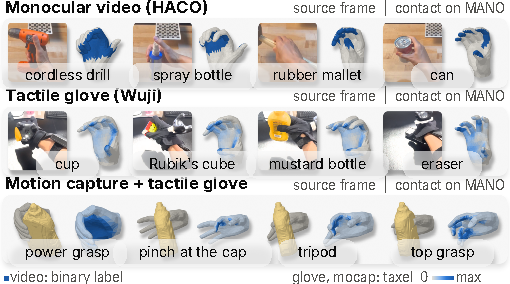
\includegraphics[width=\linewidth]{figs/fig_data_gallery_1col.pdf}
    \caption{\textbf{Demonstration sources.} We show some demonstration exmaples from monocular video (Vid-HACO contact), tactile glove (taxel pressure), and motion capture with the tactile glove  (taxel pressure).
}
    \label{fig:gallery}
\end{figure}

\begin{figure}[t]
    \centering
    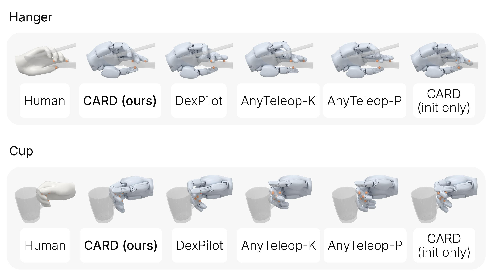
\includegraphics[width=\linewidth]{figs/fig_baselines_1col.pdf}
    \caption{\textbf{Contact-anchored vs.\ kinematic retargeting} on two video clips. Per clip: the human source, \ours, DexPilot, AnyTeleop-K, AnyTeleop-P, and \ours's geometric initialization (init only), the columns of \cref{tab:contact_quality}. The scanned object is for visualization only, and orange spheres are the \fcas. Kinematic baselines reach the object but do not track the contact.}
    \label{fig:baselines}
\end{figure}


\subsection{Replay: Tactile Tracking Controller}
\label{sec:method:replay}

\begin{figure}[t]
    \centering
    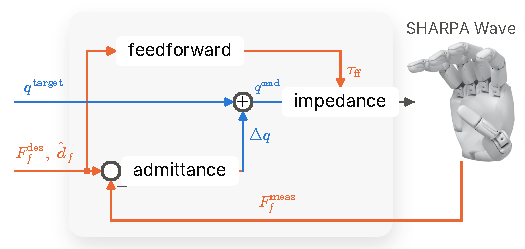
\includegraphics[width=0.85\linewidth]{figs/fig_tracker_diagram.pdf}
    \caption{\textbf{Tactile tracker.} Each finger uses fingertip force feedback to track the desired contact force through an admittance loop whose curls form the joint offset $\Delta q$, while feedforward torque directly applies the target force through the joint impedance controller (\cref{app:tracker}).}


    \label{fig:tracker_diagram}
\end{figure}

The retargeting pipeline outputs a joint trajectory $q^{\mathrm{target}}$ and, per finger $f$, a desired normal force $F^{\mathrm{des}}_f$ along the push direction $\hat{d}_f$. A tactile controller tracks both (\cref{fig:tracker_diagram}). An integral-dominant admittance on the error between $F^{\mathrm{des}}_f$ and the measured fingertip normal force $F^{\mathrm{meas}}_f$ produces a scalar \emph{curl} $\kappa_f \in [0,1]$ (\cref{eq:admittance} in \cref{app:tracker}), which closes the finger along a fixed unit synergy $\hat{\psi}_f$. The summed closures form a joint offset $\Delta q = \textstyle\sum_f \kappa_f\,\hat{\psi}_f$ that updates the joint target, $q^{\mathrm{cmd}} = q^{\mathrm{target}} + \Delta q$, while a feedforward torque injects the desired force through the fingertip Jacobian $J_f$ into the joint impedance controller with gains $K_p, K_d$:
\begin{equation}
\label{eq:controller}
\begin{aligned}
\tau &= K_p\,(q^{\mathrm{cmd}} - q) + K_d\,(\dot{q}^{\mathrm{cmd}} - \dot{q}) + \underbrace{k_{\mathrm{ff}}\, J_f^{\top} F^{\mathrm{des}}_f\, \hat{d}_f}_{\tau_{\mathrm{ff}}}.
\end{aligned}
\end{equation}
Because the joints are compliant, the curl adds a bounded squeeze rather than a rigid displacement. A contact state machine freezes the integrator on sensor dropouts and arms the feedforward (gains in \cref{app:tracker}).

% The retargeted output is a joint trajectory \emph{plus} a per-finger desired force (from human demonstration), and we close the loop by using tactile tracking controller to simultaneously track the joint and the finger contact force targets. The Sharpa Wave measures the normal contact force with the tactile sensors at fingertips, an integral-dominant admittance law turns the normal-force error into a scalar \emph{curl} $\kappa_f \in [0,1]$ that update the joint target of each finger's PD controller. Along with this, we inject feedforward joint torque calculated from desired force through the fingertip Jacobian (\cref{app:tracker}) to each joint. Replay is otherwise open-loop, with no object pose estimate and no policy, so it succeeds exactly when the retargeted contacts and forces are faithful.

\subsection{Cross-Embodiment Transfer}
\label{sec:method:embodiment}

Because \fca are parameterized in the unified representation, transfer to a new embodiment needs only a \emph{semantic map} (\cref{fig:semantic_map}, \cref{app:details}). Defined anchors, cost groups, and weights can be used across embodiments. Five-fingered hands map one-to-one, region to link. Hands with fewer fingers map many-to-one, for instance, the Unitree Dex3-1 receives the middle, ring, and pinky regions on its third finger, with simultaneous anchors merged into a force-weighted centroid, and a parallel-jaw gripper maps the thumb to one jaw and the four fingers to the other. We show four embodiments' semantic mapping in \cref{fig:real,fig:embodiments}.

%===============================================================================
